\documentclass[10pt,letterpaper]{article}
\usepackage[utf8]{inputenc}
\usepackage{amsmath}
\usepackage{amsfonts}
\usepackage{amssymb}
\usepackage{graphicx}
\usepackage{tabularx}
\usepackage[left=2cm,right=2cm,top=2cm,bottom=2cm]{geometry}
\author{Trent Baker, Marie Morin, Carie Pointer}
\title{CSCI 440 - ER Diagrams}
\pagenumbering{gobble}
\begin{document}
\maketitle

A brief description of each of the relationships and entities in our ER diagram.

\noindent
\begin{tabularx}{\textwidth}{c X}
	altTitles & Other names the Title could be known as \\
	episodeOf & Reference to the parent Title of a TV show\\
	scored & The ratings a Title scored \\
	worksOn & A Crew is a collection of people who work on the Title \\
	describe & Describe holds information about people including known for, list of characters etc. \\
	AKAs & The entity that contain the alternate title \\
	Episode & The entity that contains the episode information \\
	Ratings & The entity that contains the rating information \\
	Crew & The entity that contains the Crew information \\
	Peron & An entity that contains some relevant information about a person like name, profession, notable works, etc \\
	Principals & The entity that contains the Title descripion informaiton. tConst and nConst together make the primary key for a principal
\end{tabularx}

\noindent
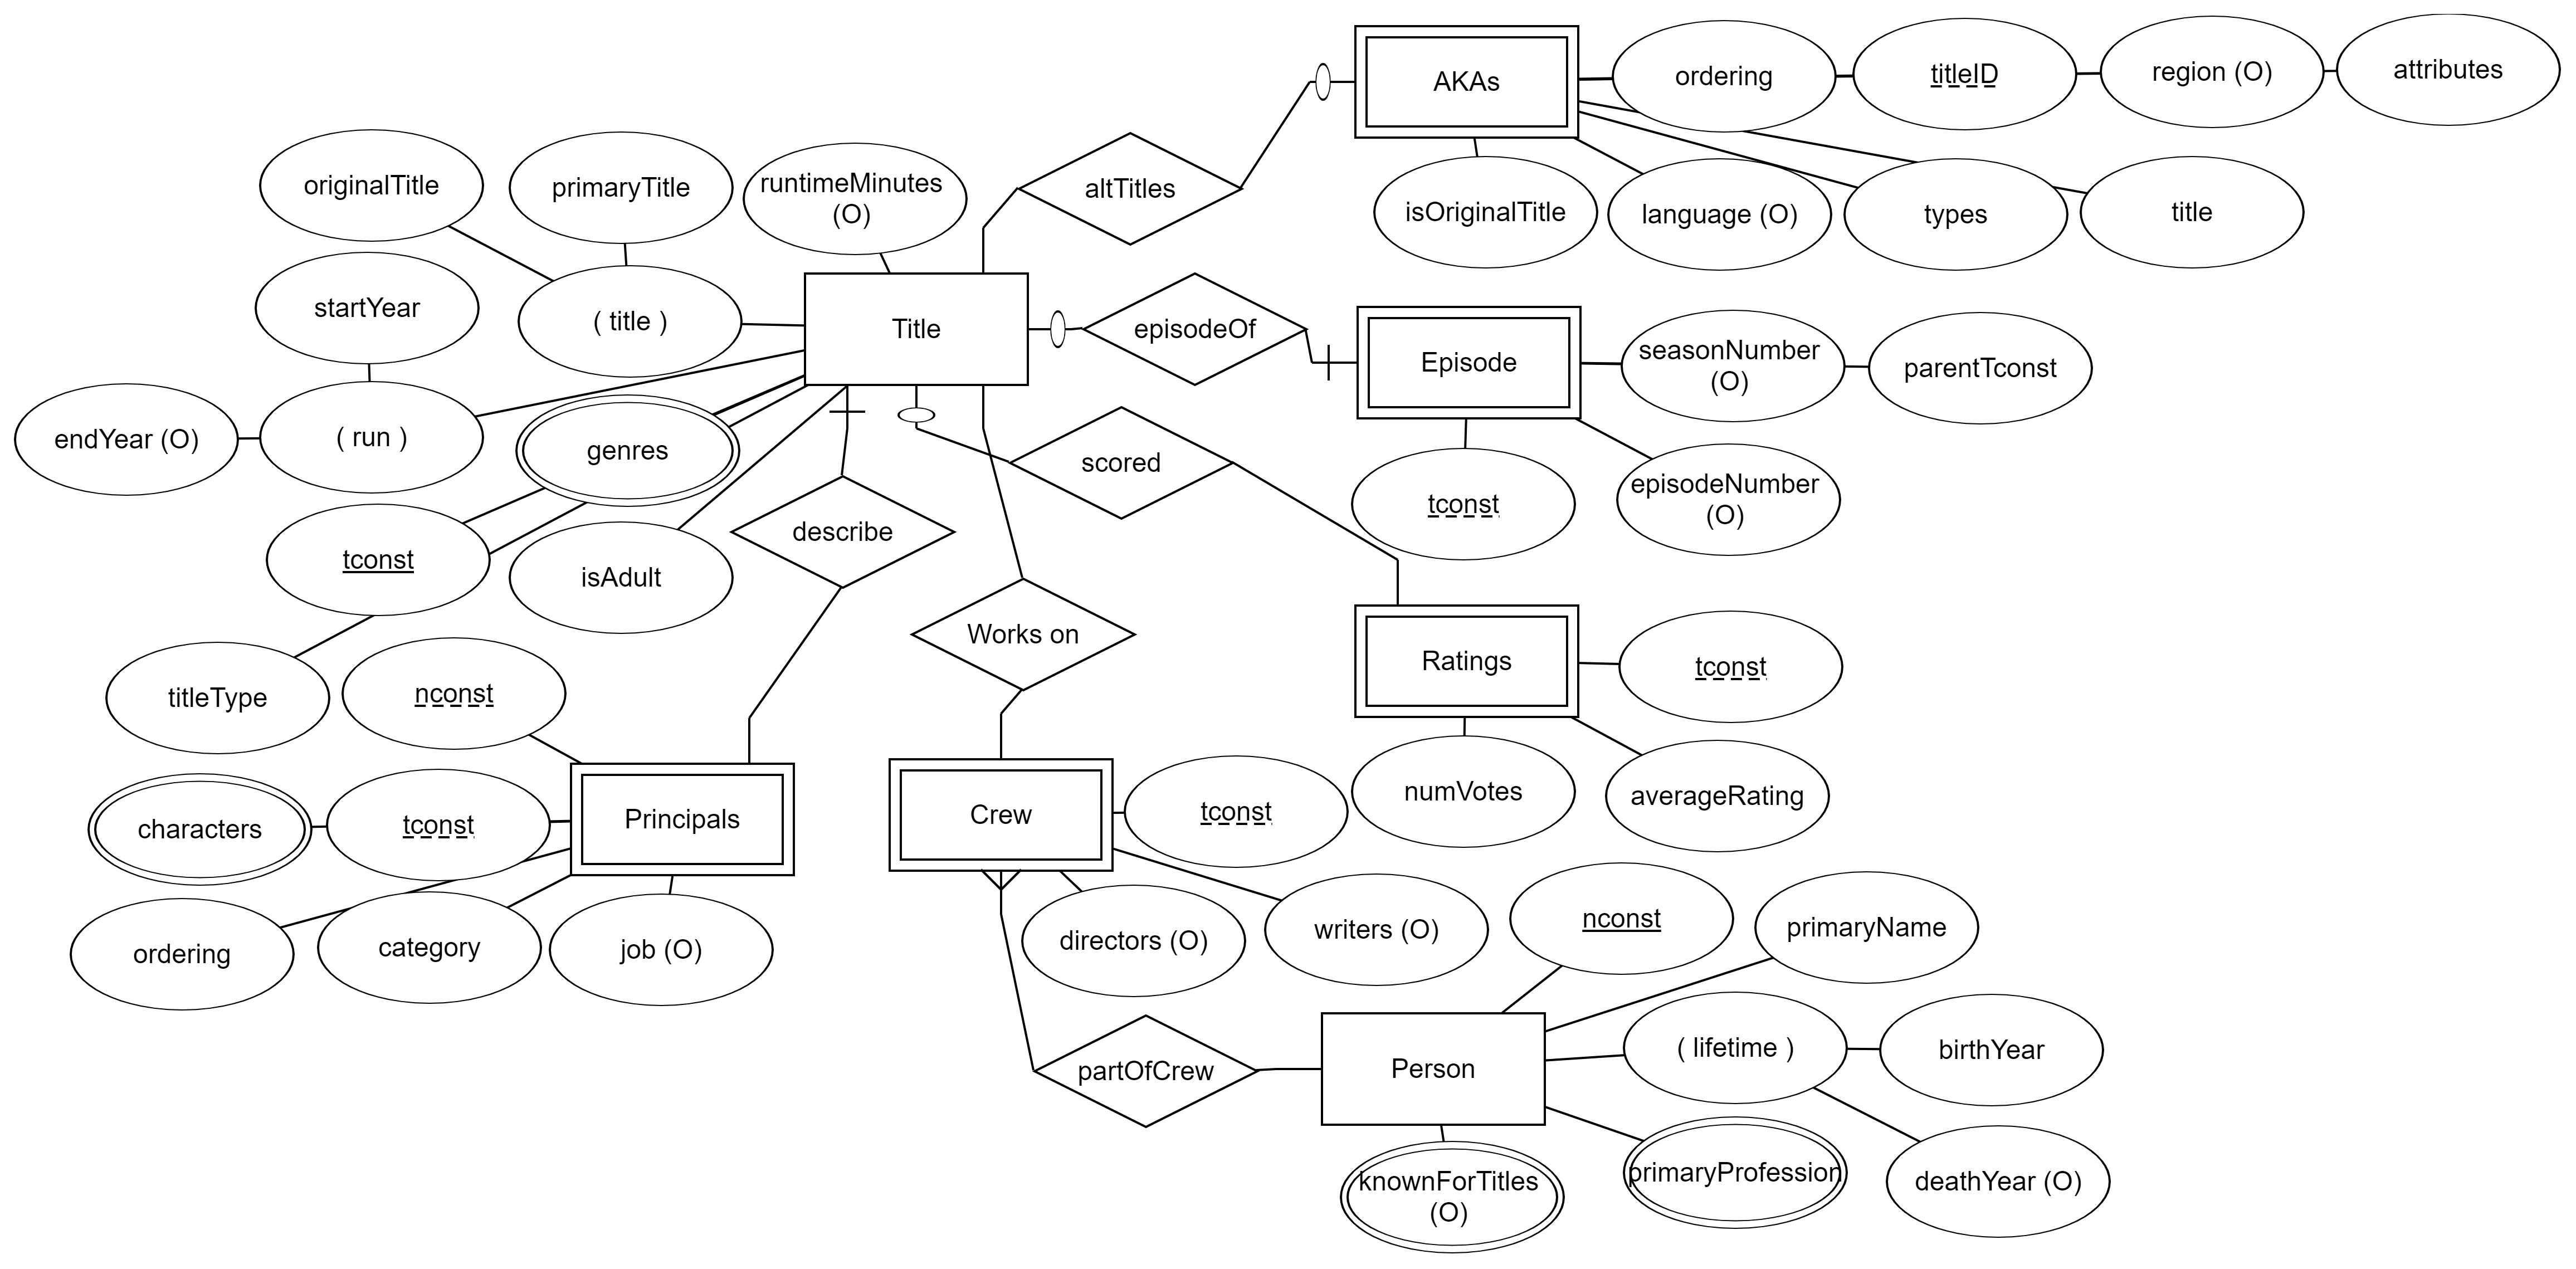
\includegraphics[width=\textwidth]{part1}

%FIX PAGE BREAKS BEFORE POSTING
\end{document}
